\chapter{Project Time Plan}
\label{ch:Project Time Plan}

In this section, the time plan for the project is discussed. This provides an overview of different tasks and what the team achieves for the course of one year. The intention of this timeline is to provide a rough idea regarding the tasks and their duration. The actual plan will be decided and defined as the project proceeds further. For better understanding, the main tasks of the project are divided as shown in the table below.

\begin{table} [h]
\centering
	\begin{tabular}{|c|l|c|c|}
	\hline
		Sr.No. & Tasks & Start & End\\
		\hline
		1 &	Project organization & 11.10.2018 &	10.11.2018\\
		\hline
		2 &	Preparation and Presentation of mini seminar & 11.10.2018 &	19.11.2018\\
		\hline
		3 &	Developing Project Plan & 20.11.2018 & 06.12.2018\\
		\hline
		4 &	Reviewing Technologies & 20.11.2018 & 20.12.2018\\
		\hline
		5 &	Designing Architecture &	06.12.2018 & 31.01.2019\\
		\hline
		6 & Implementation and Deployment &	07.02.2019 & 30.08.2019\\
		\hline
		7 & Presentation &	01.09.2019 & 20.09.2019\\
		\hline
	\end{tabular}
\caption{List of all tasks in the time plan}
\end{table}

The following list further defines the goals of each task: 
\begin{enumerate}
	\item \textbf{Project organization:}
	Establish communication between team members and understand each other, in terms of their skill-set and expertise. Also, decide upon tools for project management, task management, version control and a platform for all further communications. As an outcome, Github is used for issue tracking, task management and version control, Texstudio for documentation and Slack for internal communication.
	\item \textbf{Preparation and Presentation of mini-seminar:}
	To get an overview of various technologies and subjects that are required for the project. Select one of the subjects, research the subject in depth and present the concepts that are relevant to the project, to the team.
	\item \textbf{Developing project plan:}
	Consolidate all the seminar topics presented by each team member and make a basic sketch of what to achieve, how to achieve and by when to achieve. For the project group, the document is a valuable reference to get an overview of the problem, related technologies, and required sub-tasks. 
	\item \textbf{Reviewing technologies:}
	To list all the technologies that are relevant to the project, review the pros and cons of each technology and to decide upon technologies to be used in the project.
	\item \textbf{Designing architecture:}
 The aim is to discuss, design and document the base for implementation. The project group has been divided into sub-groups and the sub-groups will decide on technologies and methods/approaches for implementation. The sub-groups are as follows.
 
\begin{table} [h]
	\centering
	\begin{tabular}{|c|c|c|}
		\hline
		WP1 & WP2 & WP3 \\
		\hline
		Arkajit & Sanket & Ashwin \\
		\hline
		Vivek &	Harshitha & Bhargavi \\
		\hline
		Suheel &  & Deeksha \\
		\hline
	\end{tabular}
	\caption{Details of sub-groups}
\end{table}
	
	This phase is one of the most crucial phases in the project group, as it is a core foundation to the project.
	\item \textbf{Implementation and Deployment:}
	 Each sub-group works independently on the respective work packages and shares the updates with the team on weekly basis. Integration and testing the end product by benchmarking and defining various test cases to be able to deliver a stable product by the end of the implementation phase. This requires maximum efforts and time, as various versions/prototypes will be developed until a satisfying and stable end product is obtained. Implementation can be done in the following stages.
	
		\begin{itemize}
		\item\textbf{Initial Development}: Sub-groups working independently on respective work packages.
		\item\textbf{Unit Test}: Conduct testing on each of the packages developed.
		\item\textbf{Integration}: Integrate the work of all the sub-groups.
		\item\textbf{Final Testing}: Use bench-marking and test the final product. 	
	\end{itemize}


	\item \textbf{Presentation:}
	After implementing the software suite, it is presented to the supervisors. This is achieved by presenting the results obtained in the form of a report or pictorial representation. Also, the team presents the challenges, insights, and benefits inferred from the end product that is built. 
	\end{enumerate}


\begin{figure}
	\centering
	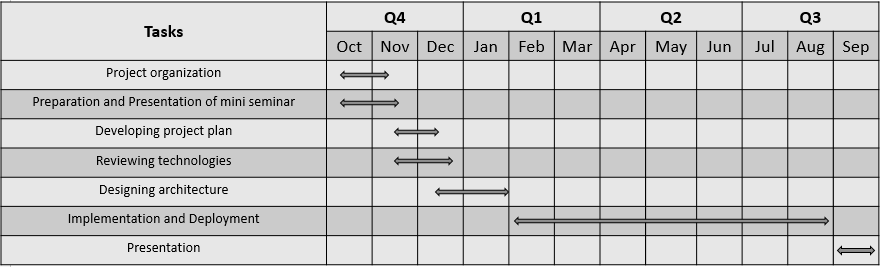
\includegraphics[width=1.0\linewidth]{figures/timeplan}
	\caption{A gantt diagram visualizing the time plan.}
	\label{fig:timeplan}
\end{figure}

The sequence of tasks is visualized in the above diagram. Though the timeline mentioned is fixed and can change during the course of various phases of the project, this is to constantly remind the team about the deadlines and to foresee further responsibilities and milestones to be achieved. 


	